%\documentclass[twocolumn]{emulateapj}
%\documentclass[12pt,preprint]{aastex}

\documentclass[usenatbib]{mn2e}



\newcommand{\s}{$_{\rm s}$}
\newcommand{\kms}{km~s$^{-1}$}
\newcommand{\msun}{{\it M}$_{\odot}$}
\newcommand{\lsun}{{\it L}$_{\odot}$}
\newcommand{\mear}{{\it M}$_{\oplus}$}
\newcommand{\etal}{{\it et al.}}
\newcommand{\ie}{{\it i.e.}}
\newcommand{\eg}{{\it e.g.}}
\newcommand{\be}{\begin{equation}}
\newcommand{\ee}{\end{equation}}
\newcommand{\magarc}{{\rm mag\,arcsec$^{-2}$}}
\newcommand{\MK}{{{\rm M}_{\rm ext,K}-5\log h}}
\newcommand{\ri}{{$r_{21}$}}
\newcommand{\ra}{$R_A$}
\newcommand{\vobs}{{v_{\rm obs}}}
\newcommand{\kmsMpc}{km~s$^{-1}$ Mpc$^{-1}$}
\newcommand{\h}{$h_{70}$}
\newcommand{\vpec}{v_{\rm pec}}
\newcommand{\like}{{\mathcal L}}
\newcommand{\vs}{\vspace*{5pt}}
\newcommand{\continued}{ (Continued)}

% Journals
\newcommand{\mnras}{MNRAS}
\newcommand{\apj}{ApJ}
\newcommand{\apjl}{ApJL}
\newcommand{\aj}{AJ}
\newcommand{\pasp}{PASP}
\newcommand{\aaps}{A\&AS}
\newcommand{\aap}{A\&A}
\newcommand{\apjs}{ApJS}
\newcommand{\araa}{ARA\&A}
\newcommand{\pbar}{p_{\rm bar}}
\newcommand{\fHI}{f_{\rm HI}}

%\shorttitle{Galaxy Zoo View of the Hubble Sequence}
%\shortauthors{Masters \etal}

\voffset-1.25cm

\usepackage{epsfig}
\begin{document}

%\title{The Galaxy Zoo View of the Hubble Sequence}
%\author{Galaxy Zoo Team} 
%\altaffiltext{1}{ICG}
%\altaffiltext{2}{Harvard-Smithsonian Center for Astrophysics, 60 Garden Street, Cambridge, MA 02138}
%\altaffiltext{3}{MIT}
%\altaffiltext{4}{??}
%\email{kmasters@cfa.harvard.edu}

\title[Galaxy Zoo View of the Hubble Sequence]{The Galaxy Zoo View of the Hubble Sequence}
%Bars Regulating Star Formation though the Atomic Gas Content of Disc Galaxies}
%The Atomic Gas Content of Barred Galaxies from ALFALFA$^*$: Bar Feedback in Intermediate Mass Disc Galaxies }
\author[K.L. Masters \etal]{Karen L. Masters$^{1,2}$, Kyle Willett, Kevin Casteels and other Galaxy Zoo science team  \newauthor members (even if your name doesn't start with K)\\
% Robert C. Nichol$^{1,2}$, Martha P. Haynes$^3$, Chris Lintott$^4$, \newauthor Brooke Simmons$^5$, Ramin Skibba$^6$, Steven Bamford$^7$, Riccardo Giovanelli$^3$, \newauthor  Kevin Schawinski$^{5,8}$ \\
$^1$Institute for Cosmology and Gravitation, University of Portsmouth, Dennis Sciama Building, Burnaby Road, Portsmouth, PO1 3FX, UK \\
$^2$South East Physics Network, www.sepnet.ac.uk\\
%$^3$Dept. of Astronomy, Cornell University, Space Sciences Building, Ithaca, NY 14850, USA\\
 %$^2$Institute for Sciences of the Cosmos (ICCUB), University of Barcelona, Marti i Franques 1, Barcelona, 08024 Spain\\
% $^{4}$Oxford Astrophysics, Department of Physics, University of Oxford, Denys Wilkinson Building, Keble Road, Oxford, OX1 3RH, UK\\
%$^{5}$Yale Center for Astronomy and Astrophysics, Yale University, P.O. Box 208121, New Haven, CT 06520, USA \\
%$^6$Steward Observatory, University of Arizona, 933 N. Cherry Ave, Tuscon, AZ 85721, USA\\
 %$^4$Astronomy Department, Adler Planetarium and Astronomy Museum, 1300 Lake Shore Drive, Chicago, IL 60605, USA\\
 % $^7$Centre for Astronomy \& Particle Theory, University of Nottingham, University Park, Nottingham, NG7 2RD, UK\\
 %$^6$School of Physics and Astronomy, University of Minnesota, Minneapolis, MN 55455, USA\\
 %$^7$Department of Physics \& Astronomy, 206 Gallalee Hall, 514 University Blvd., University of Alabama, Tuscaloosa, AL 35487-0234, USA\\
% $^8$Einstein Fellow\\ 
\\
 $^*$This publication has been made possible by the participation of more than 200,000 volunteers in the Galaxy Zoo project. \\ Their contributions are individually acknowledged at \texttt{http://www.galaxyzoo.org/volunteers}. \\
\\
{\tt E-mail: karen.masters@port.ac.uk}
 }

%\date{Accepted for publication in MNRAS, 7th October 2010.}
%\pagerange{1--10} \pubyear{2010}

\maketitle



\begin{abstract}

We use classifications provided by citizen scientists in the Galaxy Zoo project to consider the current view of the Hubble Morphological Sequence for galaxies. 

\end{abstract}

%\keywords{galaxies: distances and redshifts --- galaxies: clusters --- galaxies: fundamental parameters --- distance scale --- cosmological parameters}

\section{Introduction}


The classification of objects into categories is a common starting point for many areas of science. Galaxy morphology (shapes and types) remains the most obvious starting point for this process in extragalactic astronomy. The morphology of a galaxy encodes information about its formation history and evolution through what it reveals about the orbits of the stars in the galaxy, and is known to correlate well with other physical properties (e.g. Roberts \& Haynes 1994). Many galaxy classification schemes have been developed (see Buta 2011, and Sandage 2005 for recent reviews), but the one first presented by Hubble (1926) remains the basis of the most commonly used schemes. The ``Hubble sequence" splits galaxies into ``spiral" and ``elliptical" types, and in addition orders the spiral galaxies in a sequence extending away from the ellipticals. By analogy with the terminology used for star classification at the time (and with no comment on evolutionary paths) Hubble dubbed these ``early" and ``late"-types, a terminology which has stuck. Here we explore an updated view of the Hubble Sequence obtained from visual classifications provided by 160,000 members of the public on $\sim$ 250,000 galaxies from the Sloan Digital Sky Survey (SDSS) Main Galaxy Sample (MGS; Strauss et al. 2002). These classification were made public as part of the SDSS DR10 (Ahn et al. 2013), and are described in detail in Willett et al. (2013)\footnote{Also see {\tt data.galaxyzoo.org}}. 

The original Hubble sequence of disc galaxies (Hubble 1926) labelled Sa-Sb-Sc (and extended to Sd by de Vaucouleurs 1959) was set up using three distinct criteria. These were based on (1) spiral arm appearance, split into (a) how tightly wound the spiral arms are and (b) how clear, or distinct the arms are, and (2) the prominence of the central bulge. Sa galaxies were described as having large bulges and tight, smooth (very distinct) arms, while in contrast a typical Sc was described as having a very small ``inconspicuous" bulge and very loose patchy (indistinct) arms. In Hubble's language ``normal" (S) and ``barred" (SB) spirals had identical parallel sequences. These types are illustrated by Hubble's own preferred examples (except for the S0 which appeared later) in Figure \ref{sequence}. 

\begin{figure}
%\includegraphics[width=84mm]{barfraction_gasfraction.ps}
\includegraphics[height=80mm,angle=-90]{TuningFork.ps}
\caption{The Hubble Sequence illustrated by the examples suggested by Hubble (1926) with images from the SDSS.  The galaxies are: : E0 � NGC 3379; E5 � NGC 4621;  Sa - NGC 4594 (``The Sombrero");  Sb - NGC 2841; Sc -  NGC 5447 (``The Pinwheel"); SBa - NGC 2859; SBb - NGC 3351 (or M95); SBc - 7479. We have also included an S0 (NGC 6278), not in Hubble�s original scheme.) \label{sequence}}
\end{figure}

Among experts in morphology (e.g. Sandage 2005, Buta 2012), there has been a consensus that for most spiral galaxies these three criteria result in consistent classification. Buta explains however, that ``in conflicting cases, emphasis is usually placed on the appearance of the arms". Examples, particularly of Sa galaxies with small bulges are described in the literature (for example - Sandage 1961, Hogg, Roberts \& Sandage 1993, Sandage \& Bedke (1994), Jore, Broeils \& Haynes 1996), and Sandage (2005) notes that the existence of ``small bulge Sa galaxies" (as defined by their arm types) had been recognised even in Hubble's time. Buta (2012) also explains that SB galaxies with nuclear rings in small bulges may commonly have tightly wound arms, and therefore be classes as Sa. 

\begin{figure}
%\includegraphics[width=84mm]{barfraction_gasfraction.ps}
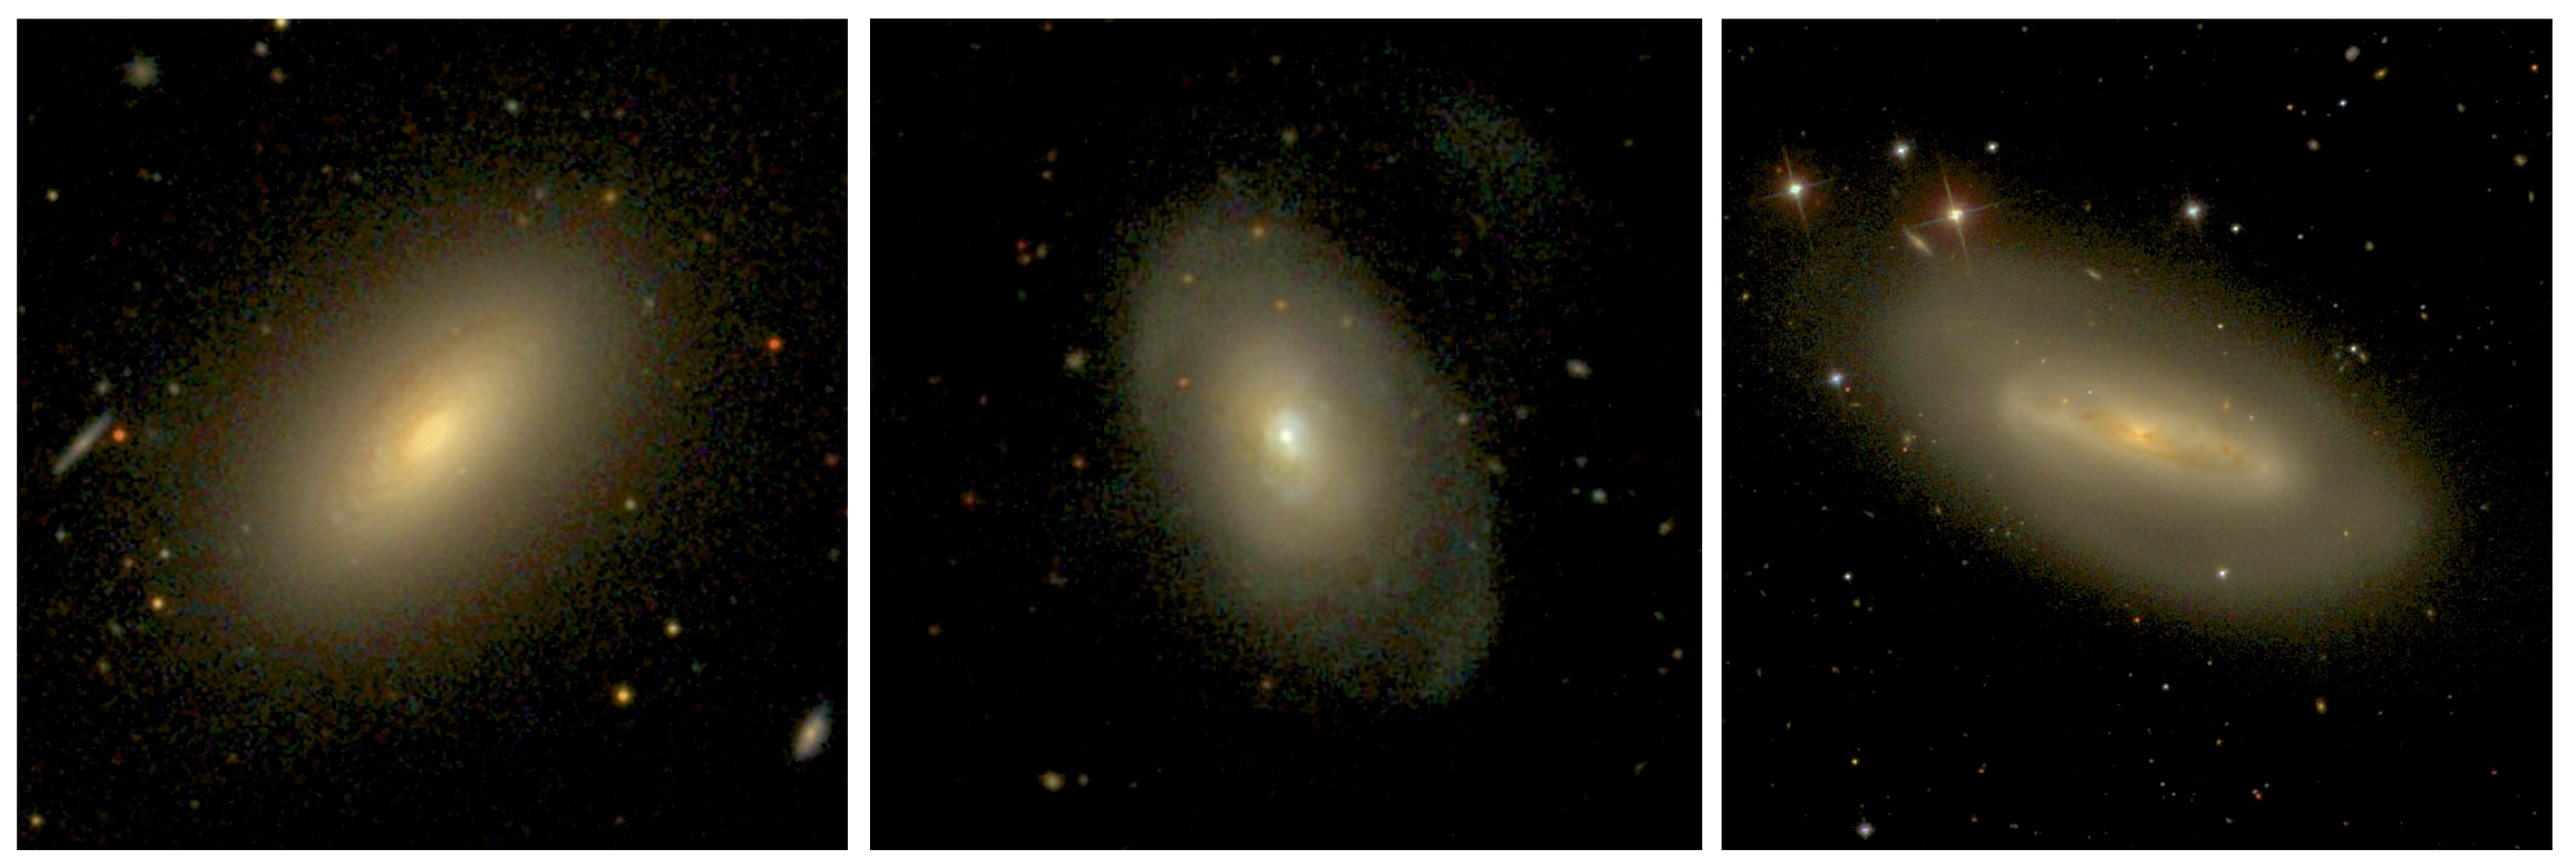
\includegraphics[height=80mm,angle=-90]{ExampleSas.ps}
\caption{Examples of Sa galaxies with large, intermediate and small bulges from the classifications by Hogg, Roberts \& Sandage (1993).  The galaxies are (from left to right) large bulge Sa: NGC 2639; intermediate bulge Sa: NGC 3604; small bulge Sa: NGC 4293\label{Sa}}
\end{figure}


However modern automatic galaxy classification has tended to conflate bulge size alone with spiral type (e.g. Lauikainen et al. 2007, Masters et al. 2010a need more), and automatic classification of galaxies into ``early-" and ``late-" types, referring to their location on the Hubble Sequence and based on $B/T$ or some proxy for this through central concentration (e.g. Sersic index, cite) has become common. Indeed, Sandage (2005) says this is not new, claiming "the Hubble system for disk galaxies had its roots in an arrangement of spirals in a continuous sequence of decreasing bulge size and increasing presence of �condensations� over the face of the image that had been devised by Reynolds in 1920"

Also see Kormendy \& Bender 2011 about the S0a, S0b, S0c sequence based on B/T alone. 
Elmegreen \& Elmegreen 1987 - classes of spirals arms from flocculent to grand design.

Discuss pseudo-bulges versus classical bulges (e.g. Fisher \& Drory)?
Talk about ATLAS-3D results on early-types? 

Obviously not yet a finished intro. 

%In Hogg et al. 1993: recent discussions of the variation of physical parameters across the Hubble Sequence (e.g. Knapp et al. 1989, Eder et al. 1991, Young \& Scoville 1991). Discusses Sas with no evidence of star formation as being "generic to the classification sequence rather than the result of environmental processes (Sandage 1983)". 

\section{Sample and Data} 

Todo: Description of Galaxy Zoo classifications pointing heavily to Willett et al. (2013). 

Todo: Cite Davis \& Hayes (2013) about the reliability of spiral arm tightness identification. Ask for their sample to make better plot that Figure \ref{pitch}, and also to calibrated $A_{\rm Winding}$ with pitch angle. 

\begin{figure}
%\includegraphics[width=84mm]{barfraction_gasfraction.ps}
\includegraphics[width=70mm]{PitchAngleDH13.ps}
\caption{Proportion of galaxies receiving majority votes for tight arms (blue), median (green) or loose arms (red) as a function of pitch angle measured by Davis \& Hayes (2013). Dashed lines are all galaxies analysed, the solid lines are galaxies with good citizen scientist agreement on classifications. This figure is reproduced from Davis \& Hayes (2013).  \label{pitch}}
\end{figure}

We select a low redshift volume limit for the main sample considered in this paper. Of the 243500 galaxies in the main spectroscopic sample of GZ2 (Willett et al. 2013), we selection $N=22118$ which are found in the redshift range $0.01<z<0.035$, and which have an $r$-band absolute Petrosian magnitude of $M_r < -19.0$. We remove eight of these galaxies which have more than 50\% of their classification votes for ``star or artefact". Inspecting these objects they are typically genuine galaxies, but with corrupted images (e.g. under a satellite trail, or diffraction spike from a nearby bright star). However, they do not have useful GZ2 classification since so many people marked them as artefacts.

Define other properties considered below. E.g. colours, stellar masses. 

\section{Frequency of Different Galaxy Zoo Morphologies}

We show in Figure \ref{sample}, the 22110 galaxies in our nearby volume limited sample on plots of $p_{\rm features}$ versus optical colour and magnitude ({\bf TODO: these are not the best way to get colour from SDSS, and also currently using DR7 not DR10}). These plots illustrate the well known tendency for galaxies to have two main morphological classes, in the GZ2 language those with features and those without, which is similar to the classic ``early-type" (meaning without spirals arms) and ``late-type" (\ie with spiral arms or other features). Note that the locus of ``featured" galaxies span the entire colour range of this volume limited sample, while ``smooth" galaxies are predominately red (although small samples of blue ``smooth" galaxies do exist, like the blue ellitpticals of Schawinski et al. 2009). 

``Features" in the Galaxy Zoo classification tree might include disturbed or irregular morphology or mergers. Users could identify these in GZ2 after indicating the that the galaxy showed ``odd" features, and then indicating what they thought was odd. All users classifying a galaxy answered this question. We select for these by requiring at $p_{\rm odd} > 0.42$ and $N_{\rm odd}>20$ (as recommended in W13), and then by requiring $(p_{\rm irregular}+p_{\rm disturbed} + p_{\rm merger} > 0.6$ (ie. aproximately 60\% or more of the classifiers thought the galaxy was either irregular, disturbed or merging). As users could select only one of these options, using the sum is the most reliable way to identify all such objects. We find that $N=1362$ (or 6\% of  the galaxies) meet these criteria, and of these 73 (0.3\%) are found to have the largest vote for ``merger", 411 (1.9\%)  for ``disturbed" and 848 (3.8\%) for ``irregular". As these are a small fraction of the sample removing them makes little difference to the results below, never-the-less we remove them in what follows and proceed with $N=20748$ ``normal" galaxies. 

\begin{figure*}
%\includegraphics[width=84mm]{barfraction_gasfraction.ps}
\includegraphics[width=160mm]{sample_features.ps}
\caption{Shown are plots of $p_{\rm features}$ versus absolute magnitude and optical colour, as well as a classic colour magnitude diagram for the 22118 galaxies in our nearby volume limited sample from Galaxy Zoo 2. This illustrated the known tendency for galaxies to have two main types split by both colour and magnitude. \label{sample}}
\end{figure*}

 Using thresholds of $p_{\rm smooth}>0.8$ and $p_{\rm features}>0.8$ to identify cleanly classified galaxies we find that 39\% of galaxies in the sample are clearly ``featured", and 13\% are clearly ``smooth", (the remaining 48\% have only lower consensus classifications). Relaxing this to find the majority answer for all galaxies in the sample we find 63\% of the normal galaxies are best identified as ``featured" and 37\% as ``smooth". Random examples of these two classes at $z=0.03$ (the median redshift of the sample) and as a function of absolute magnitude are shown in Figure \ref{examples}. In Willet et al. (2013) we recommend thresholds of $p_{\rm smooth}>0.469$ and $p_{\rm features}>0.430$, with a minimum classifier count of $N=20$ to identify samples of galaxies in which classifications from further down the classification tree will  be reliable. We find 39\% of the sample ($N=8063$) pass this smooth threshold and 46\% ($N=9610$ pass it for featured), leaving 15\% ($N=3075$ galaxies) with only basic classifications. Table \ref{basic} summarises these data, and in addition includes fractions for galaxies in subsets by their absolute magnitude which demonstrates the well known tendency for brighter (or more massive galaxies) to be more likely to be ``smooth". 
 
\begin{table*}
\caption{Distribution of basic morphological class\label{basic}}
\begin{tabular}{lccccc}
\hline\hline
Sample/defintion &  $N_{\rm smooth}$ & \%$_{\rm smooth}$ & $N_{\rm featured}$ & \%$_{\rm features}$\\
\hline
All ($N=22118$) \\
~~~~~~~~~ $p>0.8$ & 2695 & 13 & 8053 & 39 \\
~~~~~~~~~ $p>0.5$ & 7859 & 38 & 13069 & 63 \\
~~~~~~~~~ Majority vote & 7751 & 37 & 12993 & 63 \\
~~~~~~~~~ W13 criteria  & 8063 & 39 & 9610 & 46 \\
Majority vote  \\
~~~~~~~~~ Faint $M_r > -20$ ($N=10483$) & 3744 & 39 & 5896 & 61 \\
~~~~~~~~~ Mid 1 $-21< M_r < -20$ ($N=7609$) & 2436 & 34 & 4802 & 66 \\
~~~~~~~~~ Mid 2 $-22< M_r  < -21$ ($N=3553$) & 1318 & 38 & 2105 & 62 \\
~~~~~~~~~ Bright $M_r < -22$ ($N=465$) & 253 & 57 & 190 &  43\\
\hline\hline
\end{tabular}
\end{table*}

\begin{figure*}
%\includegraphics[width=84mm]{barfraction_gasfraction.ps}
\includegraphics[width=160mm]{example1.ps}
\caption{Randomly selected example images of galaxies classified as either ``featured" (top row) or ``smooth" (bottom row) from Galaxy Zoo as a function of $r$-band absolute magnitude (brighter to the right).  All galaxies have a redshift $z=0.03$ and are shown at the same angular scale. Images are $gri$ composites from SDSS with a scale of 1.7\arcmin square. {\bf Add an intermediate or uncertain row}. \label{examples}}
\end{figure*}

\subsection{Visibility of Spiral Arms and Bars}
 
 Among the galaxies identified as ``featured" and with enough classifications at the next questions, we find 16\% ($N=1498$) have values of $p_{\rm edge on}>0.8$. This is consistent with the number of galaxies expected to be found with $i=100\deg$ in a completely randomly orientated sample of objects. The recommended threshold for ``oblique" galaxies in which we can reliably identify disc features (e.g. bars, spirals; Willett et al. 2013) is $p_{\rm not edge on}>0.715$ (and $N_{\rm not edge on}>20$). We find that 71\% of the ``featured" galaxies fall into this group ($N=6858$). 
 
 Of these oblique featured galaxies: 
\begin{itemize}
\item 78\% have clear spiral arms ($p_{\rm spiral} > 0.5$) and just 7\% are found to not have spiral arms to a high consensus ($p_{\rm spiral}<0.2$). 
\item 26\% have obvious bars ($p_{\rm bar}>0.5$). This strong bar fraction is consistent with previous Galaxy Zoo based work (e.g. Masters et al. 2011, Masters et al. 2012), given the differences in sample selection. Weaker bars can be identified by $0.2<p_{\rm bar}<0.5$ (e.g. Willett et al. 2013, Skibba et al. 2011). Another 22\% of the oblique spirals have weak bars by this definition, leaving just over 50\% of oblique spirals without any clear sign of a bar feature (\ie~ $p_{\rm no bar}>0.8$) at the scales detectable by the SDSS images. 
\end{itemize}
 
 Examples of oblique galaxies with and without spiral arms and bars are shown in Figure \ref{examples2} for galaxies randomly selected from these groups at $z=0.03$. 
\begin{figure}
%\includegraphics[width=84mm]{barfraction_gasfraction.ps}
\includegraphics[width=80mm]{examplespiral_bar.ps}
\caption{Examples of galaxies with (top row from left to right) $p_{\rm bar}>0.5$,  $0.2<p_{\rm bar}<0.5$ and $p_{\rm bar}<0.2$ and (bottom row from left to right) $p_{\rm spiral}>0.5$,  $0.2<p_{\rm spiral}<0.5$ and $p_{\rm spiral}<0.2$. The exact values of these debased classification fractions are indicated.   Images are $gri$ composites from SDSS with a scale of 1.7\arcmin square.  \label{examples2}}
\end{figure}


\subsection{The Correlation of Bulge Size and Spiral Arm Tightness}

The classic Hubble Sequence for spiral galaxies suggests that bulge size and spiral arm winding are highly correlated in most cases. In this section we investigate how tightly correlated bulge size and spiral arm tightness are found to be for galaxies with visible spiral arms in the Galaxy Zoo sample. We define a unique value of bulge size and spiral arm tightness from the GZ2 classifications as: 
\be
B_{\rm size} = 0.0 ~p_{\rm no bulge} + 0.2p_{\rm  just} + 0.8p_{\rm obvious}+ 1.0~p_{\rm dominant}
\ee
and
\be
A_{\rm Winding} = 0.0 ~p_{\rm loose} + 0.5 p_{\rm medium} + 1.0 p_{\rm tight}
\ee
such that these numbers increase from zero to one for either bulge sizes increasing, or arms getting tighter (note that I inverted the arms index from what Casteels et al. in prep. is using in order than a ``classic" Sa would have both values of 1.0, and a ``classic Sc" would have both values of zero). 

 We can plot these values only for the subsample of Galaxy Zoo galaxies which have reliable classifications for both - \ie. those galaxies with visible spiral arms. We select this sample (as advised by Willett et al. 2013) using cuts on the classification votes in answers earlier up the GZ2 tree, specifically $p_{\rm features} >  0.430$,  $p_{\rm notedgeon} >  0.715$,  $p_{\rm visiblearms} >  0.619$, and in addition require the number of people answering the question about spiral arm windiness to be at least 20. This gives a sample of $N=4471$ spiral galaxies in which we can ask how well bulge size correlates with spiral arm winding angles. 
 
 We plot the measure of bulge size versus arm windiness for this sample in Figure \ref{bulgewinding}. In this volume limited ($M_r<-19$) sample of nearby ($z<0.035$) galaxies we find no strong correlation between bulge size and arm windiness. There is a slight tendency spirals with large bulges to have only tightly wound spirals (\ie. both $A_{\rm winding}$ and $B_{\rm size}$ are large), but for spirals with small bulges all values of spiral arm winding are found.  This is consistent with the previous literature, in that Sa galaxies (as defined by arm winding) have been discussed with both large and small bulges, while Sc galaxies (as defined by loose arms) are only ever discussed with small bulges. 
 
 \begin{figure}
%\includegraphics[width=84mm]{barfraction_gasfraction.ps}
\includegraphics[width=80mm]{bulgewinding.ps}
\caption{We show here the location of 4471 nearby spiral galaxies on a plot of bulge size versus degree of arm winding as indicated by Galaxy Zoo classifications. The contours indicate regions of high density of points, with points themselves shown at the lowest density.   \label{bulgewinding}}
\end{figure}

 We have checked a closer sample ($0.01<z<0.25$), and also a sample of only the brightest spirals ($M_r < -21$) and find no significant difference in the result, except for a tendency for the brighter spirals to have larger bulges, as expected. 
 
 We also split the sample based on bar classification, finding that spirals with strong bars ($p_{\rm bar}>0.5$)  were more likely to have larger bulges and less tightly wound spirals than those with no bars ($p_{\rm bar} < 0.2$), but there remains no clear correlation in either subgroup (see Figure \ref{bars}). The correlation between bars and spiral arm tightness is explored more in Casteels et al. in prep. 
 
 \begin{figure}
%\includegraphics[width=84mm]{barfraction_gasfraction.ps}
\includegraphics[width=40mm]{bulgewinding_nobars.ps}
\includegraphics[width=40mm]{bulgewinding_bars.ps}
\caption{As Figure \ref{bulgewinding} but for subsamples of the oblique spirals split by bar classification.  Left panel: galaxies with $p_{\rm bar} < 0.2$; right panel: galaxies with $p_{\rm bar} > 0.5$ \label{bars}}
\end{figure}

 Figure \ref{windingexample} shows examples of galaxies at $z=0.03$ from the four quadrants of Figure \ref{bulgewinding} with strong bars ($p_{\rm bar}>0.5$) or no bar ($p_{\rm bar} < 0.2$)
 
 \begin{figure*}
%\includegraphics[width=84mm]{barfraction_gasfraction.ps}
\center
\includegraphics[width=160mm]{examplebulgewinding2.ps}
\caption{Example images of galaxies at $z=0.03$ and $M_r\sim -21$ with both loose and tightly would spiral arms (lower and upper rows respectively) and small or large bulges (left and right columns respectively). In each case galaxies are shown with either strong bars, or no bar. Images are $gri$ composites from SDSS with a scale of 1.7\arcmin square.  \label{windingexample}}
\end{figure*}
 
\section{Constructing a Hubble Sequence from Galaxy Zoo}

% In this context we define a ``Hubble Sequence" as a sequence of galaxies in which the average physical properties vary systematically from ``early" (defined as low current star formation rates) to ``late" (defined as high current star formation rates). We consider optical colour as a proxy for SF (what about dust)..... 
 
 In W13 we discussed how best to assigned $T$-types to Galaxy Zoo galaxies from the classification votes in GZ2. Both the votes for tightness of spirals arms, and bulge size were considered. In that work we concluded that modern expert visual classification of spiral Hubble types (based on comparison with either Nair \& Abraham 2010, or Baillard et al. 2013) was primarily based on bulge size, regardless of the tightness of spiral arms, with the best fitting relation (based on symbolic regression) being found to be
 \be
 T = 4.63 + 4.17~p_{\rm no bulge} - 2.27~p_{\rm obvious} - 8.38~p_{\rm dominant}
 \ee 
 
We reproduce here the lower panel of Figure 19 from W13 which compares the predicted T-types from the above equation to the T-types assigned by Nair \& Abraham (2010). As was point out in W13, this, and other comparisons with recent expert visual classifications (e.g. the EFIGI sample of Baillard et al. 2011) demonstrates that the modern spiral Hubble sequence is defined by bulge size alone, with little reference to spiral arm tightness. 

\begin{figure}
%\includegraphics[width=84mm]{barfraction_gasfraction.ps}
\includegraphics[height=80mm,angle=-90]{T-typeW13.ps}
\caption{Predicted T-type classifications as fit by Willett et al. 2013 for GZ2 galaxies shown versus their T-types from Nair \& Abraham 2010. Galaxies are colour coded by their morphologies as identified by NA10. Galaxies shown are only those with sufficient answers to characterize the arms winding and arms number GZ2 tasks, which selects heavily for late-type galaxies. This explains the lack of ellipticals in the plot, but highlights the fact that S0 galaxies do not agree well with the linear sequence. Reproduced from Willet et al. 2013.  \label{T-type}}
\end{figure}


\section{Summary}

We present the morphological make-up of a sample of bright ($M_r <-19$), nearby ($0.01<z<0.035$) galaxies with classifications from the Galaxy Zoo project. We find that 94\% of these galaxies show the ``normal" morphologies found on the classic Hubble sequence, with 6\% classified as irregular, disturbed or merging. 

Among the ``normal" galaxies we find the typical correlation between magnitude, colour and morphology, such that ``smooth" (or ``early-type") galaxies are more common in the luminous red part of the diagram, where they make up ~50\% of the galaxies. Galaxies showing ``features" (or ``late-types") are found at all colours and magnitudes, and especially dominate the less luminous, bluer parts of the sample where they make up to two-third of the galaxies. 

 We find that the fraction of edge-on spirals is as expected for a sample of randomly orientated discs, and define a sample of ``oblique" spirals which are face-on enough for disc features to be identified. Among these 26\% have strong bars, and 50\% have no bars. The majority have clearly identified spirals (78\%), with only 7\% with a clear consensus for lacking spiral arms. These are likely S0 types with rings or bars. 

Among the spiral galaxies, we find little or no correlation between spiral arm winding tightness and bulge size. Although spirals with large bulges are found to typically have tightly wound  arms, those with small bulges are found with a much wider range of spiral arm pitch angle. We find that the presence of a strong bar tends to correspond to more loosely wound arms and larger bulges. 

 We demonstrate that modern expert visual classification has moved away from the classic ``Hubble sequence" which prioritised spiral arm angles over bulge size (leading to discussion of small bulged Sa galaxies) and is now predominately an ordered on central bulge size. Something about how this makes sense for a sequence on star formation since bulge size correlates so well with star formation in discs...? 
 
  Some interpretation of what the degree of arm winding actually means. 
 
\paragraph*{ACKNOWLEDGEMENTS.} 

This publication has been made possible by the participation of more than 200,000 volunteers in the Galaxy Zoo project. Their contributions are individually acknowledged at \texttt{http://www.galaxyzoo.org/volunteers}. Galaxy Zoo 2 was developed with the help of a grant from The Leverhulme Trust.

We thank the contributors to the Galaxy Zoo Forum NGC Catalogue List \\(www.galaxyzooforum.org/index.php?topic=280028.0) for making finding SDSS images of NGC galaxies easy. 

Funding for the SDSS and SDSS-II has been provided by the Alfred P. Sloan Foundation, the Participating Institutions, the National Science Foundation, the U.S. Department of Energy, the National Aeronautics and Space Administration, the Japanese Monbukagakusho, the Max Planck Society, and the Higher Education Funding Council for England. The SDSS Web Site is http://www.sdss.org/. 

The SDSS is managed by the Astrophysical Research Consortium for the Participating Institutions. The Participating Institutions are the American Museum of Natural History, Astrophysical  Institute Potsdam, University of Basel, University of Cambridge, 
Case Western Reserve University, University of Chicago, Drexel University, Fermilab, the Institute for Advanced Study, the Japan 
Participation Group, Johns Hopkins University, the Joint Institute for Nuclear Astrophysics, the Kavli Institute for Particle Astrophysics and Cosmology, the Korean Scientist Group, the Chinese Academy of Sciences (LAMOST), Los Alamos National Laboratory, the Max-Planck-Institute for Astronomy (MPIA), the Max-Planck-Institute for Astrophysics (MPA), New Mexico State Uni- 
versity, Ohio State University, University of Pittsburgh, University of Portsmouth, Princeton University, the United States Naval Observatory and the University of Washington. 


\begin{thebibliography}{}
\bibitem[Ahn et al.(2013)]{2013arXiv1307.7735A} Ahn, C.~P., Alexandroff,  R., Allende Prieto, C., et al.\ 2013, arXiv:1307.7735 %DR10
\bibitem[Baillard et al.(2011)]{2011A&A...532A..74B} Baillard, A., Bertin, E., de Lapparent, V., et al.\ 2011, \aap, 532, A74 
\bibitem[Buta et al.(2007)]{BCO07} Buta, R.~J., Corwin, H.~G., \& Odewahn, S.~C.\ 2007, The de Vaucouleurs Altlas of Galaxies, edited by Ronald J.~Buta, Harold G.~Corwin and Stephen C.~Odewahn.~ISBN-13 978-521-82048-6 (HB).~Published by Cambridge University Press, Cambridge, UK, 2007.
\bibitem[Hubble (1926)]{Hubble1926} Hubble, E., 1926, \apj, 64, 321 %Hubble classification
\bibitem[Nair \& Abraham(2010a)]{NA10a} Nair, P.~B., \& Abraham, R.~G.\ 2010a, \apj S, 186, 427 (NA10) %classifications
\bibitem[Sandage (2005)]{S05} Sandage, A., 2005,\araa, 43, 581
\bibitem[Strateva et al.(2001)]{2001AJ....122.1861S} Strateva, I., et al.\ 2001, \aj, 122, 1861 %colour bi-modality
\bibitem[Strauss et al.(2002)]{MGS} Strauss, M.~A., Weinberg, D.~H., Lupton, R.~H., et al.\ 2002, \aj, 124, 1810 %SDSS Main Galaxy Sample.
\bibitem[de Vaucouleurs (1956)]{dV56} de Vaucouleurs, G.\ 1959, Handbuch der Physik, 53, 275 
\bibitem[de Vaucouleurs et al. (1991)]{RC3} de Vaucouleurs, G., de Vaucouleurs, A., Corwin, H.~G., Jr., Buta, R.~J., Paturel, G., \& Fouqu{\'e}, P.\ 1991, Third Reference Catalogue of Bright Galaxies,~ Springer, New York, NY (USA).


\end{thebibliography}

\end{document}
